%! Author = denis
%! Date = 28.06.2026

% Preamble
\documentclass[11pt,aspectratio=169]{beamer}

% Packages
\usepackage{amsmath}
\usepackage{booktabs}
\usepackage{graphicx}

\usetheme{Madrid}
\usecolortheme{seahorse}
\setbeamertemplate{navigation symbols}{}

\title[Tremor Analysis]{Do Tremors Appear at Different Times\\and with Different Intensities?}
\subtitle{Digital Biomarker -- Scientific Question}
\author[]{Denis Schatzmann}
\institute[]{FHNW -- Medical Software Development}
\date{\today}

% Document
\begin{document}

% ---------------------------------------------------------------------------
% Slide 1 -- Scientific question
% ---------------------------------------------------------------------------
\begin{frame}{1. Scientific Question}
    \begin{block}{}
        \textbf{Do tremors appear periodically and with different
        intensities?}
    \end{block}

    \vspace{1em}
    \begin{itemize}
        \item Tremor: a shaking movement, is a digital biomarker
        \item Idea: it comes in episodes, not constantly
        \item Measure with a smartphone
    \end{itemize}
\end{frame}

% ---------------------------------------------------------------------------
% Slide 2 -- Sensors
% ---------------------------------------------------------------------------
\begin{frame}{2. Sensors Used}
    Smartphone (Pixel 8 Pro) with the Sensor Data Collection App.

    \vspace{1em}
    \begin{itemize}
        \item \textbf{Gyroscope}: measures rotation
        \item \textbf{Linear acceleration}: measures motion
    \end{itemize}

    \vspace{1em}
    Both react strongly to shaking, so they capture tremor well.
\end{frame}

% ---------------------------------------------------------------------------
% Slide 3 -- Analytics
% ---------------------------------------------------------------------------
\begin{frame}{3. Analytics}
    \begin{columns}[c]
        \begin{column}{0.55\textwidth}
            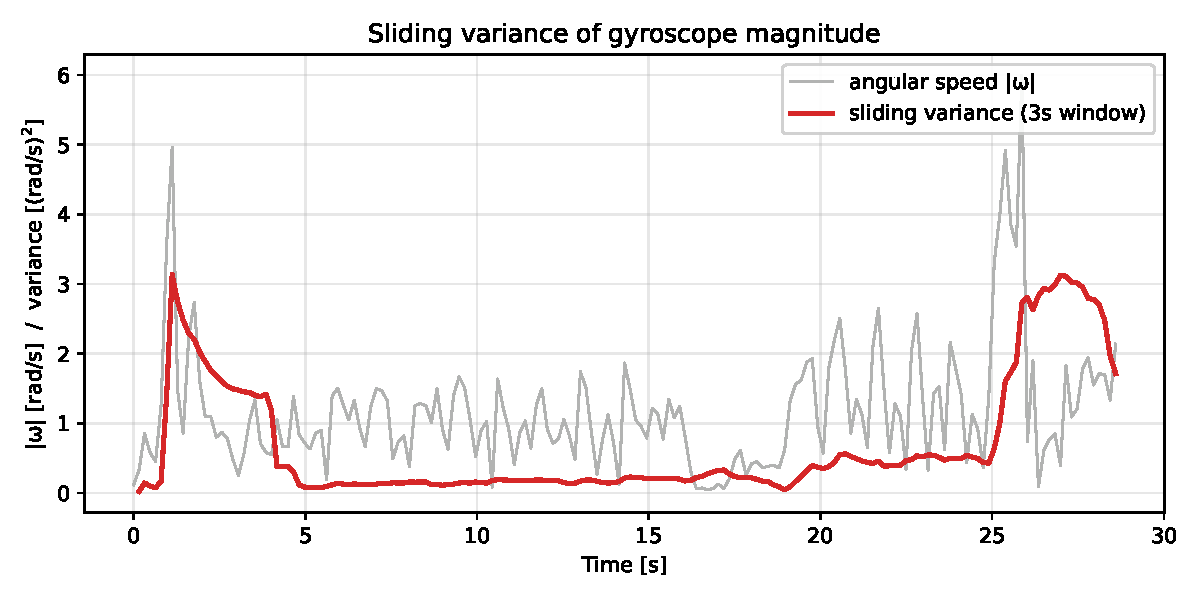
\includegraphics[width=\linewidth]{figures/sliding_variance.pdf}
        \end{column}
        \begin{column}{0.45\textwidth}
            \textbf{Process}
            \begin{itemize}
                \item Record sensor data over a long period (hours/days)
                \item Compute the sliding variance to find episodes
            \end{itemize}

            \vspace{0.8em}
            \textbf{Validation}
            \begin{itemize}
                \item Patients keep a journal
                \item Compare the measured episodes with their experience
            \end{itemize}
        \end{column}
    \end{columns}
\end{frame}

\end{document}
